\begin{table*}[t]
\centering
\caption{Certified bracket for the smallest cap with $\delta_b<0.025$. A lower endpoint $l$ means every cap below $l$ is certified insufficient; the upper endpoint has a feasible approximation below the tolerance. Equality identifies this minimum exactly.}
\label{tab:budgetthresholds}
\small
\setlength{\tabcolsep}{4pt}
\begin{tabular}{llrrr}
\toprule
Model & Output & Seed & Minimum cap LB & Minimum cap UB \\
\midrule
GBDT & probability & 20261108 & 4 & 5 \\
MLP & probability & 20261108 & 7 & 9 \\
GBDT & threshold & 20261108 & 6 & 6 \\
MLP & threshold & 20261108 & 10 & 10 \\
GBDT & probability & 20261109 & 4 & 5 \\
MLP & probability & 20261109 & 7 & 9 \\
GBDT & threshold & 20261109 & 7 & 9 \\
MLP & threshold & 20261109 & 10 & 10 \\
GBDT & probability & 20261110 & 4 & 6 \\
MLP & probability & 20261110 & 7 & 9 \\
GBDT & threshold & 20261110 & 8 & 9 \\
MLP & threshold & 20261110 & 10 & 10 \\
GBDT & probability & 20261111 & 4 & 5 \\
MLP & probability & 20261111 & 8 & 9 \\
GBDT & threshold & 20261111 & 7 & 7 \\
MLP & threshold & 20261111 & 10 & 10 \\
GBDT & probability & 20261112 & 4 & 5 \\
MLP & probability & 20261112 & 7 & 9 \\
GBDT & threshold & 20261112 & 7 & 9 \\
MLP & threshold & 20261112 & 10 & 10 \\
\bottomrule
\end{tabular}
\end{table*}
\begin{figure*}[t]
\centering
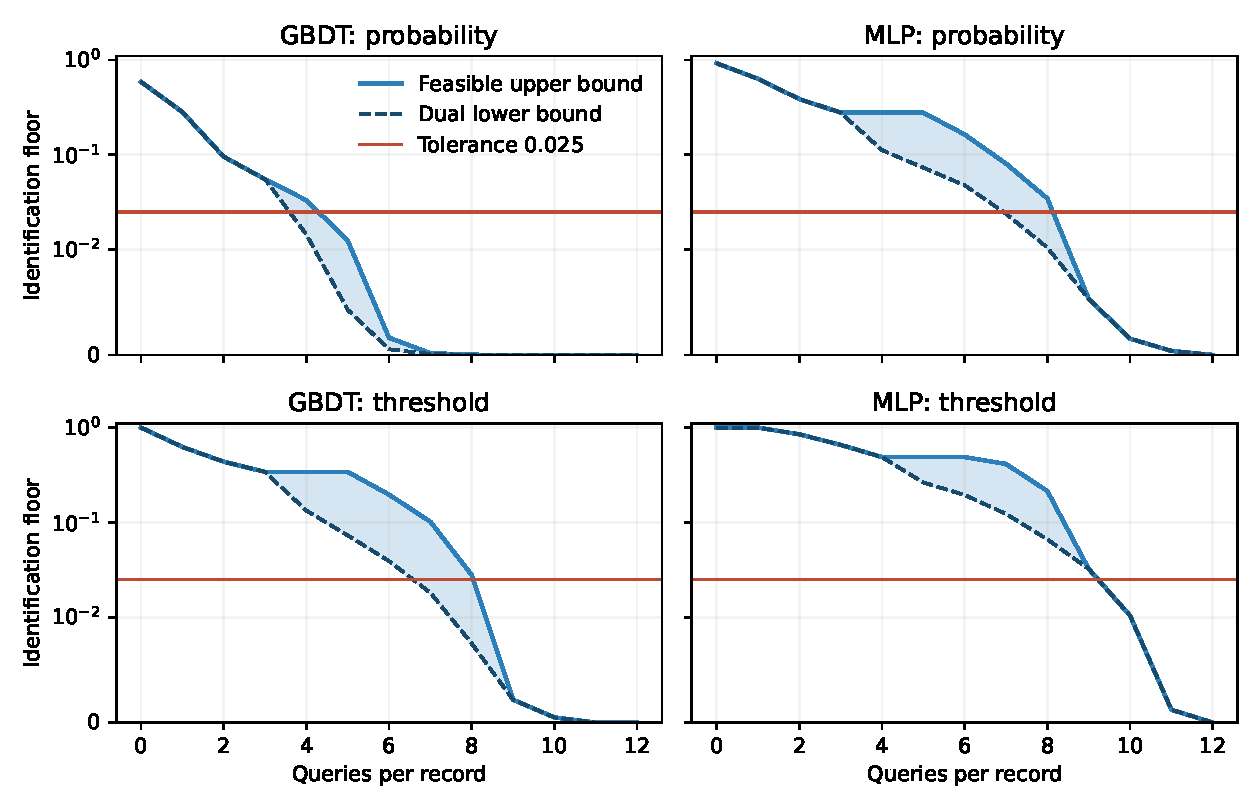
\includegraphics[width=.96\textwidth]{figures/budget_curves.pdf}
\caption{Median certified identification-floor brackets across five fixed WDBC splits. Solid curves are upper bounds, dashed curves lower bounds, and shading shows the remaining uncertainty. The horizontal line is the target 0.025. Upper and lower medians need not come from the same split. The vertical scale is linear below 0.01 and logarithmic above.}
\label{fig:budgetcurves}
\end{figure*}
